\section{Analysis Detail}
In this section, we will discuss the analysis detail, in this analysis, the event plane method is used to calculate the directed flow ($v_{1}$)and elliptic flow ($v_{2}$). By following the standard event plane method, firstly we discuss the event plane reconstruction from TPC(Time Projection Chamber) and EPD(Event Plane Detector), TPC's $\eta$ coverage is [-1,1], and the EPD is located at the forward rapidity region, $\eta$ $\in$ (-5.1, -2.1). Since it is Fixed target model collision in this analysis, the acceptance of final state particle is not symmetric around midrapidity, we cannot use 2-sub event method to calculate the resolution, which is commonly used in the BES-I collider model collision, the 2-sub event method requires each sub-event has similar multiplicity and resolution. So, in this analysis, we employ 3-sub event method to calculate the resolution. After that, we will do the particle identification (PID) for pion, kaon proton, then, we introduce the $v_{1}$ and $v_{2}$ calculation.
\subsection{Event Plane Reconstruction}
We will separately introduce the first-order and second-order Event Plane Reconstruction from TPC and EPD.

In order to calculate the resolution for each event plane, we divide the TPC to 2-sub events and EPD to 4-sub events based on their pseudorapidity ($\eta$) range. In the figure \ref{fig:tpc_epd_div}, we show the schematic plot of TPC and EPD sub-events. Since this is fixed-target model collision, we only measure the negative pseudorapidity ($\eta$) region.  In the collider model, the origin point of the Lab frame is in the center of TPC , the EPD is located at $\eta$ $\in$ (-5.1, 2.1). In the fixed-target model, the origin point of the Lab frame is shifted to the edge of TPC, as a result that the $\eta$ of EPD is boosted at $\eta$ $\in$ (-5.3, -2.6).
\begin{figure}[hp]
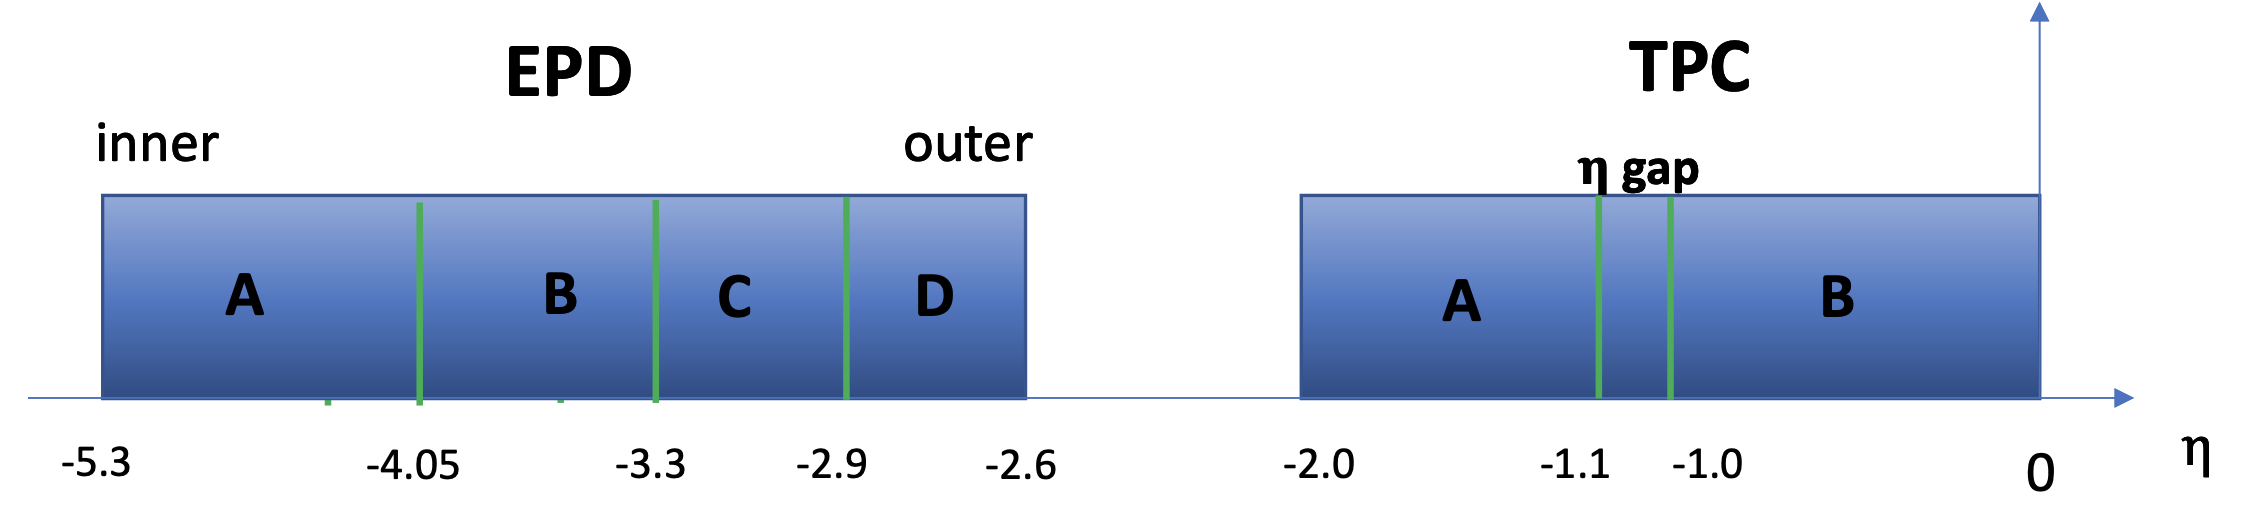
\includegraphics[scale=0.3]{chapter2/fig/tpc_epd_div.png}
\caption{The schematic plot of TPC and EPD sub-events}
\label{fig:tpc_epd_div} 
\end{figure}

\subsubsection{TPC Event Plane Reconstruction}
The event plane method correlates each particle with the event plane determined from these particles without the particle of interest, which can be done for each harmonic. Here we only discuss the first-order event plane reconstruction.
For TPC event plane, these tracks, that are required to pass the following cuts in the table \ref{tab:tpc_ep_cuts}, will be used:
\begin{table}[ht]
\caption{\ Tracks cuts for TPC event plane reconstruction}
\label{tab:tpc_ep_cuts}
\begin{tabular}{|c|c|}
\hline
-2.0$<$ $\eta$ $<$-1.1 (for TPC-A) \\ \hline
-1.0$<$ $\eta$ $<$0 (for TPC-B) \\ \hline
nHitsFit$>$15 \\ \hline
nHitsFit/nHitsMax$>$0.52 \\ \hline
dca $<$ 3 (cm) \\ \hline
0.2 $<$ $p_{T}$ $<$ 2.0 (GeV/c)\\ \hline
\end{tabular}
\end{table}
In order to calculate the first-order event plane angle, firstly we construct the Q vector from particle's azimuthal angle. And the event plane angle can be determined from the Q vector.
\begin{equation}
	\vec{\rm Q}=
	\left( \begin{array}{ccc}
		Q_{y} \\
		Q_{x}
	\end{array} \right)
	=
	\left( \begin{array}{ccc}
		\sum_{i}w_{i}sin(\phi) \\
		\sum_{i}w_{i}cos(\phi)
	\end{array} \right)
	\label{equ:Qvector}
\end{equation}

\begin{equation}
	\Psi_{1} = tan^{-1} \left( \frac{\sum_{i}w_{i}sin(\phi)}{\sum_{i}w_{i}cos(\phi)} \right)
	\label{equ:psi1_TPC}
\end{equation}

\begin{equation}
	w_{i} = 
	\begin{cases}
		p_{T}, 0.2<p_{T}<2.0 (GeV/c) \\
		2.0, p_{T} > 2.0 (GeV/c)
	\end{cases}
	\label{equ:weight_TPC}
\end{equation}

Where sums extend over all particles i used in the event plane calculation, and $\phi$ is particle azimuthal angle in the laboratory frame, and $w_{i}$ is the weight for the $i^{th}$ particle, here we use the $p_{T}$ as the weight and set the threshold of 2GeV in order to suppress the non-flow contribution on event plane reconstruction. The $\Psi_{1}$ is the first-order event plane angle. The reaction plane azimuthal angle distribution should be isotropic in the laboratory frame if the detectors have ideal acceptance. But the detectors always have non-uniform acceptance. In order to remove the acceptance correlations from the imperfect detector, we must make the event plane angle distribution isotropic or flat. A procedure for flattening the laboratory event plane angle distribution is necessary. In this analysis, we perform the re-centering and shift calibration to make the event plane angle distribution flat, it will be discussed in the following. 
\subsubsection{EPD Event Plane Reconstruction}
The event plane reconstruction using EPD is similar to TPC. While the TPC measures the tracks and EPD measures the ADC (analog-digital converter) value in each sectors. The figure \ref{fig:epd_view} shows the schematic plot of EPD (Event Plane Detector). As we can see, EPD has 16 rings, there are 24 sectors in each ring, while there are 12 sectors in the inner most ring, totally one side EPD has 372 sectors, we can measure the azimuthal angle for each sector.
As we can see, in the figure \ref{fig:epd_view}, we divide the EPD to 4 groups based on the rings. From inner to outer, EPD-A (1-4 ring), EPD-B (5-8 ring), EPD-C (9-12 ring), EPD-D (13-16 ring). We will reconstruct the event plane in these EPD groups separately. 
\begin{figure}[hp]
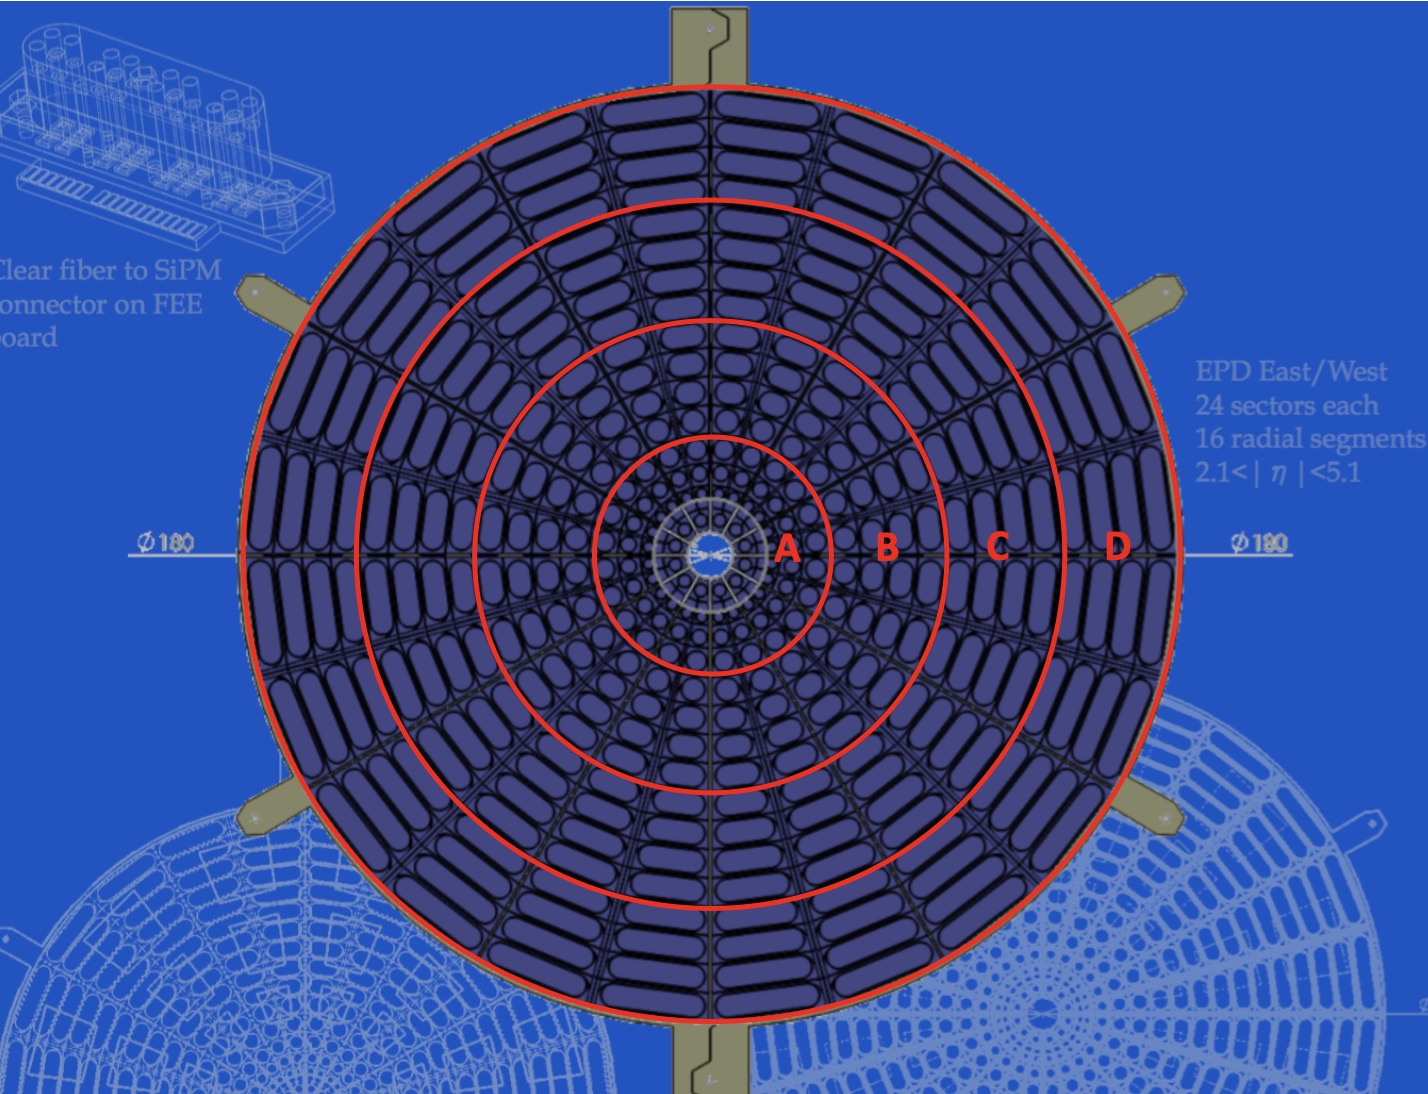
\includegraphics[scale=0.26]{chapter2/fig/epd_div.png}
\caption{The schematic plot of EPD and EPD sub-events}
\label{fig:epd_view} 
\end{figure}

For the event plane reconstruction, we firstly construct the Q vector from the aziluthal angle of sector and calculate the event plane angle from Q vector.
\begin{equation}
	\vec{\rm Q}=
	\left( \begin{array}{ccc}
		Q_{y} \\
		Q_{x}
	\end{array} \right)
	=
	\left( \begin{array}{ccc}
		\sum_{i}w_{i}sin(\phi) \\
		\sum_{i}w_{i}cos(\phi)
	\end{array} \right)
	\label{equ:Qvector_EPD}
\end{equation}

\begin{equation}
	\Psi_{1} = tan^{-1} \left( \frac{\sum_{i}w_{i}sin(\phi)}{\sum_{i}w_{i}cos(\phi)} \right)
	\label{equ:psi1_EPD}
\end{equation}

\begin{equation}
	w_{i} = 
	\begin{cases}
		nMip, 0.3<nMip<2.0 \\
		2.0, nMip > 2.0
	\end{cases}
	\label{equ:weight_EPD}
\end{equation}
Where sums goes over all hits detected by EPD, and $\phi$ is azimuthal angle of EPD sectors in the laboratory frame, and $w_{i}$ is the weight for the $i^{th}$ hits, here we use the nMip as the weight, which is the calibrated ADC value. The $\Psi_{1}$ is the first-order event plane angle. As we discussed before, we will also consider the acceptance correlations from the imperfect detector and  perform re-centering and shift calibration to make the event plane angle distribution flat. In the figure \ref{fig:epd_phi_eta_dis}, we show the EPD azimuthal angle $\phi$ and pseudorapidity $\eta$ distribution using two styles, which means 1: the $\phi$ and $\eta$ in the center position of the corresponding tile. 2: the $\phi$ and $\eta$ value in the random position of the corresponding tile. Although the two styles have different distribution, the results of resolution and $v_{1}$, $v_{2}$ value using two styles are equal.


\begin{figure}[hp]
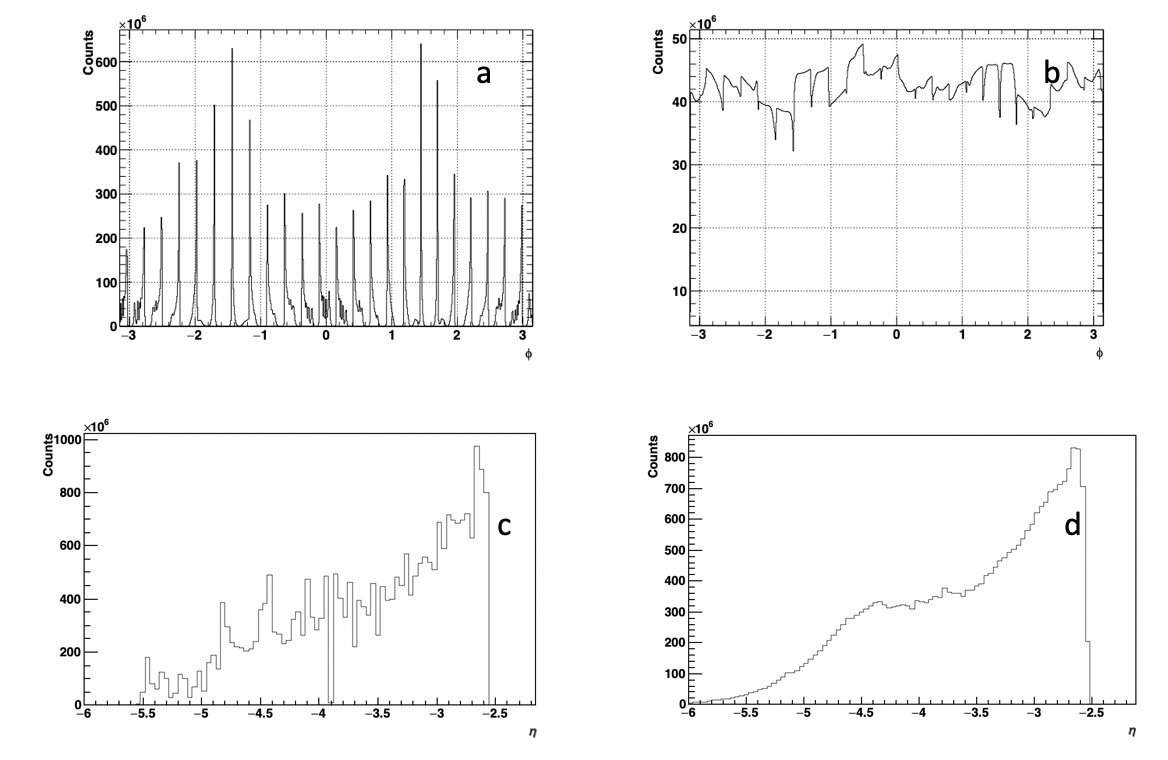
\includegraphics[scale=0.6]{chapter2/fig/epd_phi_eta.png}
\caption{Azimuthal angle ($\phi$) and pseudorapidity ($\eta$) distribution in EPD. (a): $\phi$ distribution in the center of tile, (b): $\phi$ distribution in the random of tile, (c): $\eta$ distribution in the center of tile, (d): $\eta$ distribution in the random of tile}
\label{fig:epd_phi_eta_dis}
\end{figure}

\subsubsection{re-centering and shift calibration}
The re-centering is a track-by-track calibration. One subtracts the factor from the Q-vector of each event, in which the factor is the Q-vector averaged over many events. After that, we can calculate the event plane angle. As we can see in the following equation. It is not enough that we only do the re-centering calibration. We will do the shift calibration further. The shift calibration is that one fits the non-flat distribution of $\Psi_{n}$ averaged over many events with a Fourier expansion and calculates the shifts for each event $\Psi_{n}$ necessary to force a flat distribution on average. The re-centering and shift calibration are all run-by-run and centrality-by-centrality calibration in this analysis.
\begin{equation}
	\vec{Q}_{rc} = 
	\left( \begin{array}{ccc}
	Q_{y, rc} \\
	Q_{x, rc}
	\end{array} \right)
	=
	\sum_{i}^{N} 
	\left( \begin{array}{ccc}
	w_{i}sin(\phi_{i})-\left< w_{i}sin(\phi_{i}) \right> \\
	w_{i}cos(\phi_{i})-\left< w_{i}cos(\phi_{i}) \right>
	\end{array} \right)
	\label{equ:recenter}
\end{equation}

\begin{equation}
	\Psi_{1, rc} = tan^{-1}
	\frac{Q_{y, rc}}{Q_{x, rc}}
	\label{equ:psi1_recenter}
\end{equation}

\begin{equation}
	\Psi_{1, shift} = 
	\sum_{i}^{N} \frac{2}{i}
	\left[ -\left< sin(i\Psi_{1, rc}) \right>cos(i\Psi_{1, rc})+
	\left< cos(i\Psi_{1, rc}) \right>sin(i\Psi_{1, rc})\right]
	\label{equ:shift}
\end{equation}

\begin{equation}
	\Psi_{1} = \Psi_{1, rc} + \Psi_{1, shift}
	\label{equ:psi1_shift}
\end{equation}

Where the $\vec{Q}_{rc}$ is the Q-vector after re-centering calibration, the $\Psi_{1, rc}$ is the first-order event plane angle after re-centering calibration. Then we substitute the $\Psi_{1, rc}$ into that equation to get the shift factor, the N goes $20^{th}$ order. Thus we get the flat first-order event plane angle $\Psi_{1}$.  Then we have the first-order event plane angle distribution in the figure \ref{fig:epd_tpc_psi1}, as we can see from bottom to top (TPC-A, TPC-B, EPD-A, EPD-B, EPD-C, EPD-D), from right to left (0-5\% ... 70-80\%), the black line is raw $\Psi_{1}$ distribution without any flat calibration, the blue line is the $\Psi_{1}$ distribution with re-centering calibration, it's more flat than black, the red line is $\Psi_{1}$ distribution with re-centering and shift calibration, after that, we have the isotropic or flat $\Psi_{1}$, which can correct the detector acceptance effect and be used to calculate the $v_{1}$ and $v_{2}$. We also look the correlation between different sub-events in the figure \ref{fig:epd_tpc_psi1_cor}, because we measure the same event plane in the different $\eta$ range, after fattening event plane distribution, they should have strong correlation.
\begin{figure}[ht]
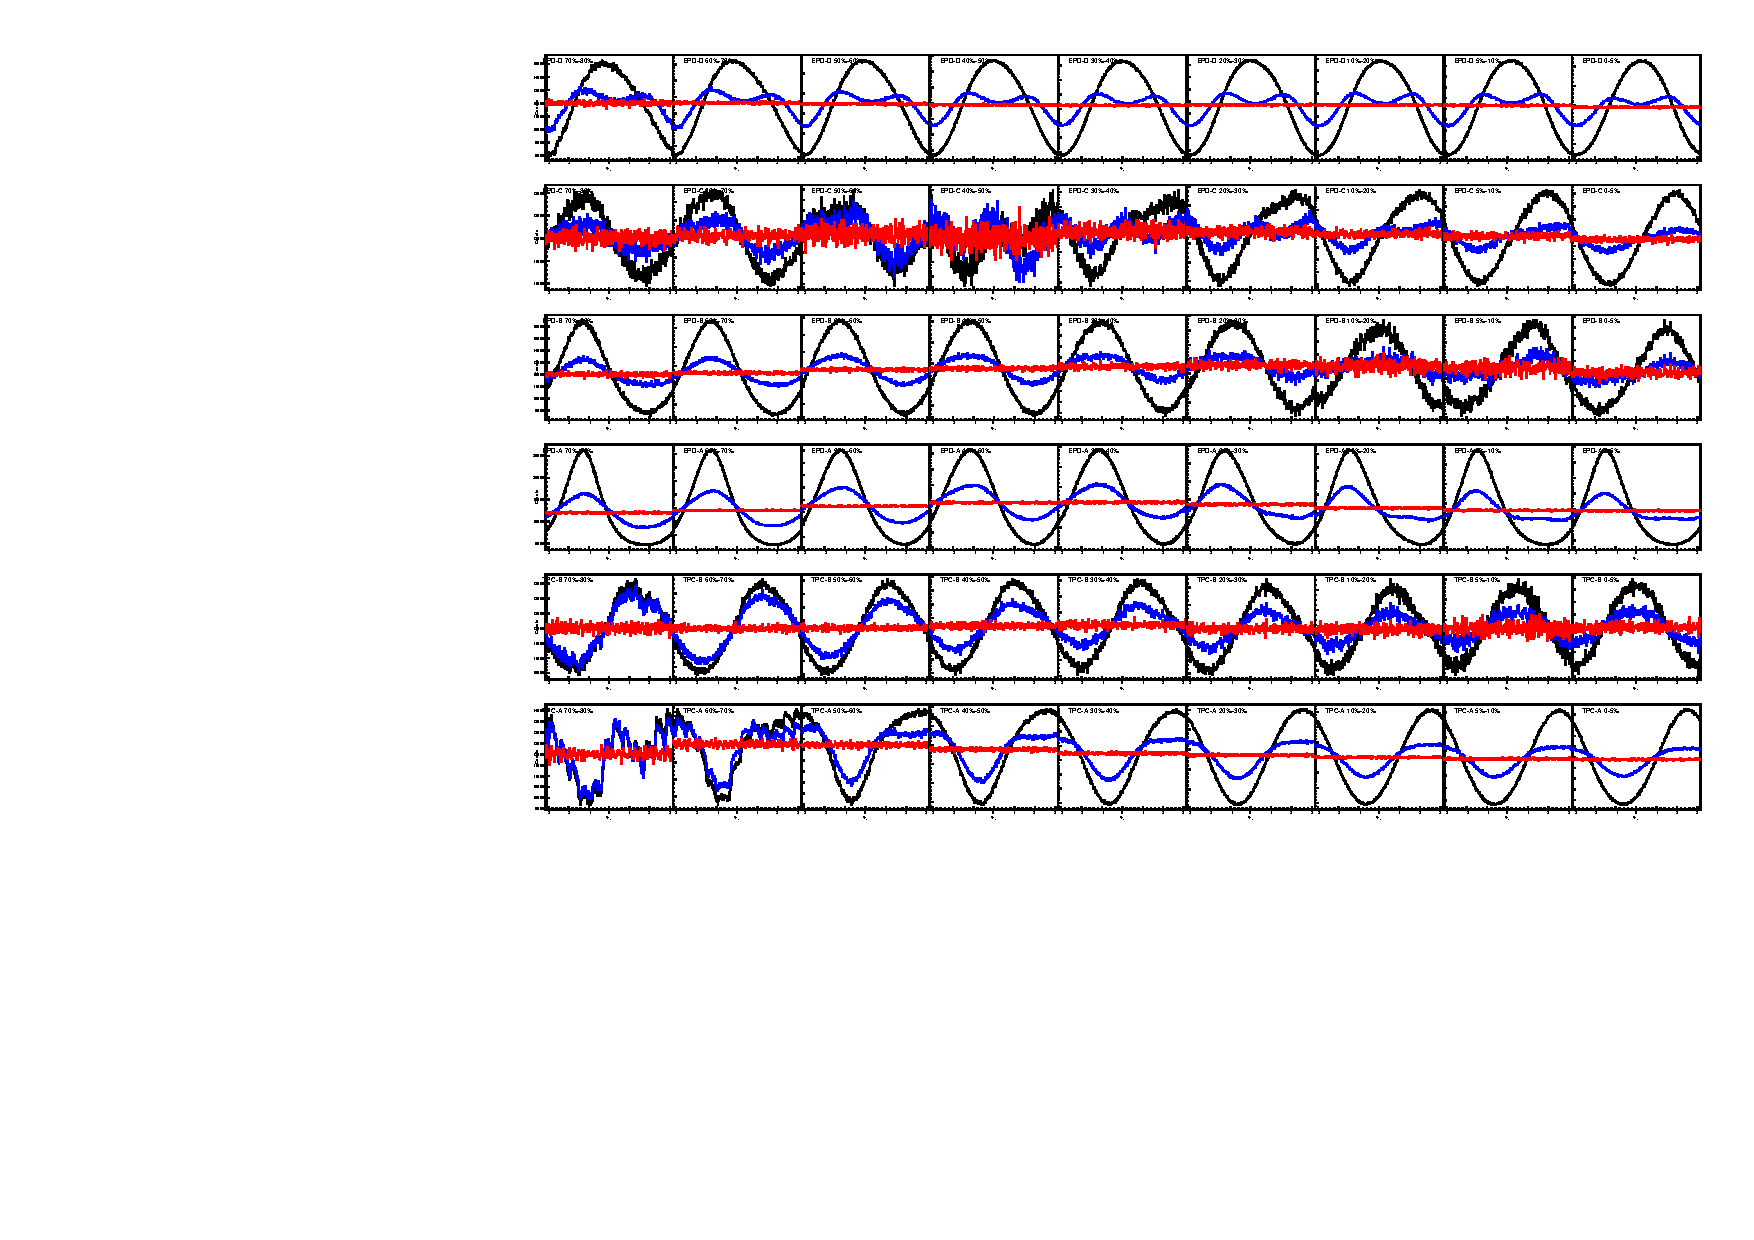
\includegraphics[scale=0.6]{chapter2/fig/epd_tpc_psi1_dis.pdf}
\caption{ TPC and EPD sub-event $\Psi_{1}$ distribution in different centrality, the black line is without raw $\Psi_{1}$ distribution, the blue line is with re-centering calibration, the red line is with re-centering and shift calibration}
\label{fig:epd_tpc_psi1}
\end{figure}

\begin{figure}[ht]
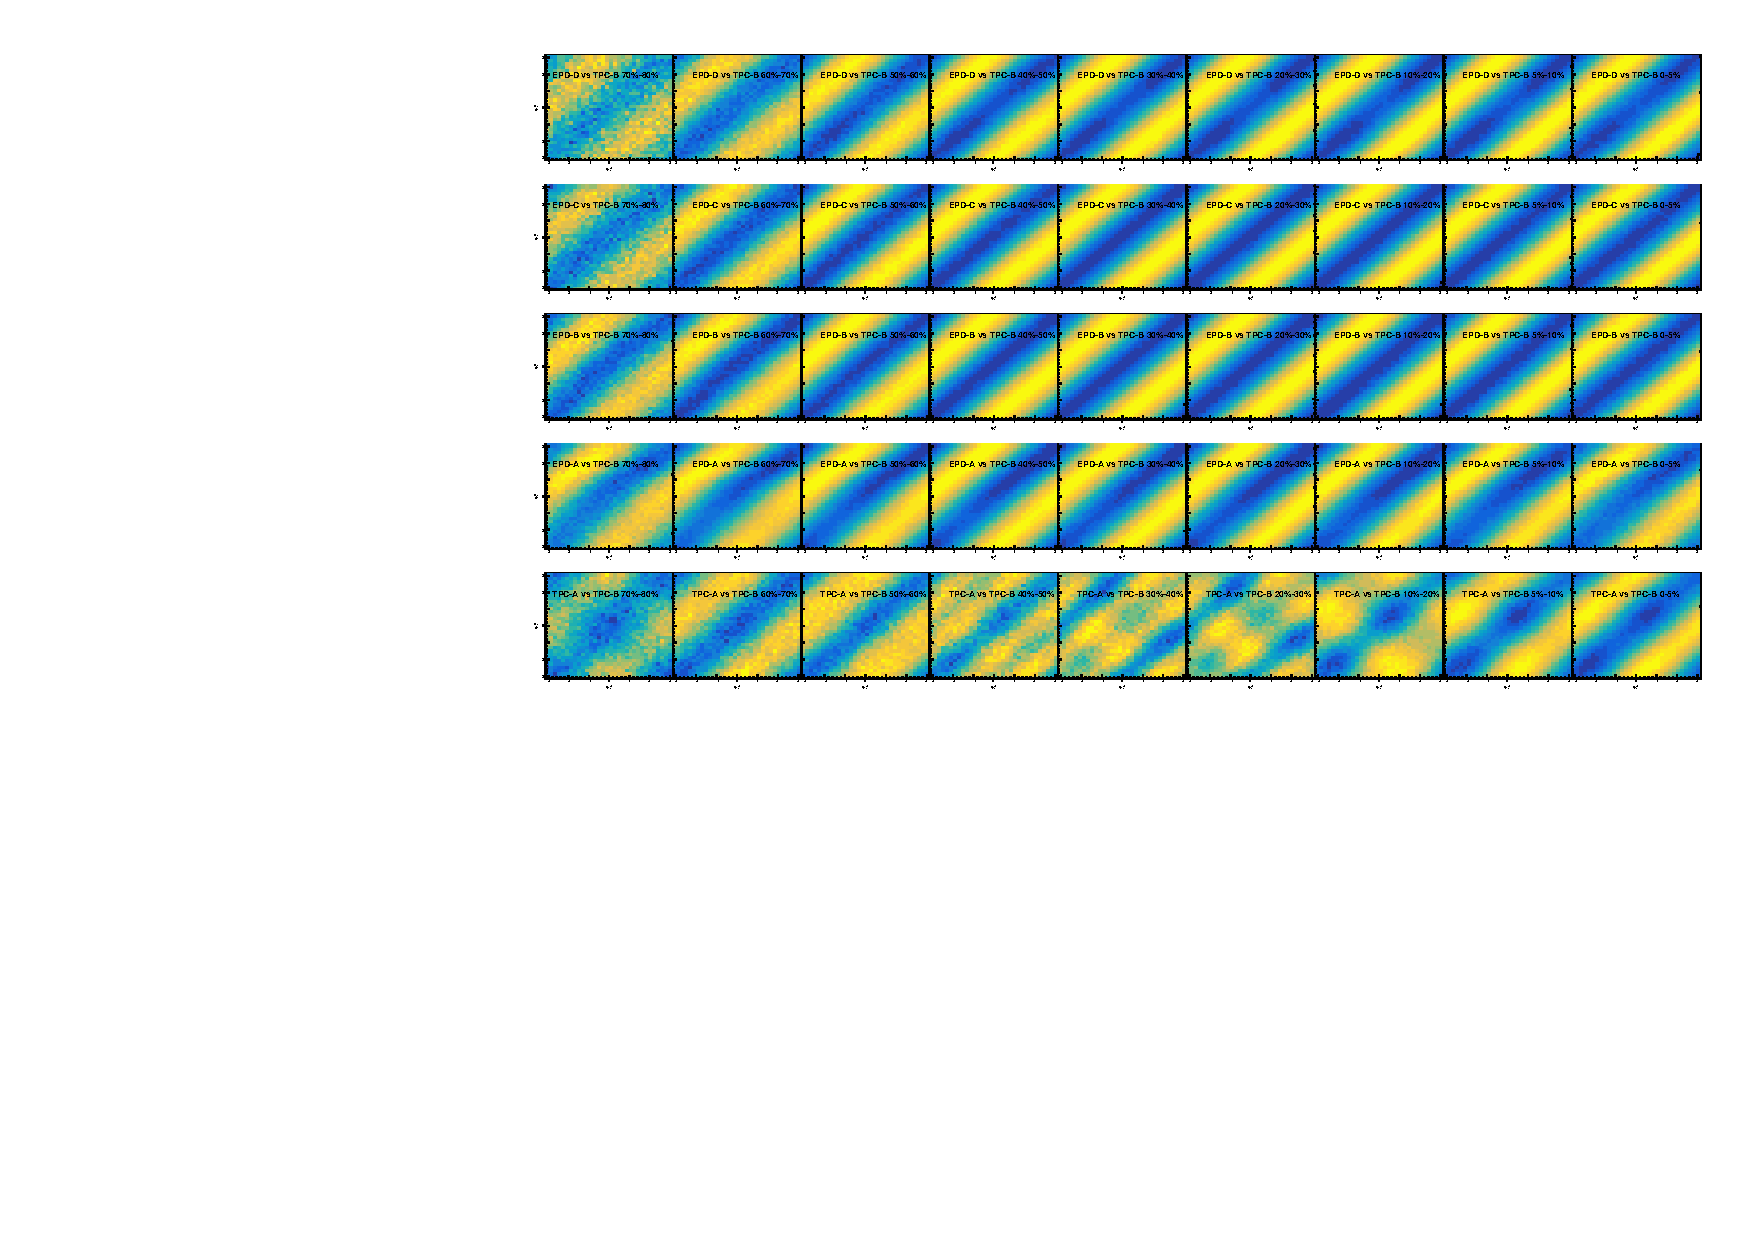
\includegraphics[scale=0.6]{chapter2/fig/epd_tpc_psi1_cor.pdf}
\caption{TPC and EPD sub-event event plane angle ($\Psi_{1}$) correlation}
\label{fig:epd_tpc_psi1_cor} 
\end{figure}


\newpage

\subsection{Event Plane Resolution}
Since the azimuthal angle of reaction plane is unknown, we use the event plane angle to estimate the reaction plane angle. Once we have the event plane angle ($\Psi_{1}$), then we can calculate the observed azimuthal anisotropy parameter ($v_{1}$, $v_{2}$). But the event plane deviates from the reaction plane, we need to correct the observed azimuthal anisotropy parameter ($v_{1}$, $v_{2}$) by event plane resolution. 
\begin{equation}
	v_{n} = \frac{v_{n}^{obs}}{R_{n}}
	=\frac{v_{n}^{obs}}{\left< cos[km(\Psi_{m}-\Psi_{r})] \right>}
	\label{equ:vn_cal}
\end{equation}
Where the $R_{n}$ is resolution, $v_{n}$ is the $n^{th}$ harmonic azimuthal anisotropy parameter, and $\Psi_{m}$ is the $m^{th}$ harmonic order event plane, k is integer number n $=$ k$*$m, $\Psi_{r}$ is reaction plane angle. The angle brackets denotes an average over all particles in all events. The event plane resolution can be expressed as:
\begin{equation}
	\left< cos[km(\Psi_{m}-\Psi_{r})] \right>=
	\frac{\sqrt{\pi}}{2\sqrt{2}}\chi_{m}exp(-\chi_{m}^{2}/4) \times
	[I_{(k-1)/2}(\chi_{m}^{2}/4)+I_{(k+1)/2}(\chi_{m}^{2})/4]
\end{equation}
Where $\chi_{m}$ $\equiv$ $v_{m}$$/$$\sigma$ and $I_{\nu}$ is the modified Bessel function of the order $\nu$. The resolution function is plotted in the figure \ref{fig:res_vs_nu}, the resolution is decreasing with k increases. Note that, numerically, when m = 1, the first order event plane angle can be used to calculate all $v_{n}$ term. In this analysis, we will use the first order event plane angle ($\Psi_{1}$) to calculate $v_{1}$ and $v_{2}$. Another reason is that, the magnitude of $n^{th}$ harmonic resolution is proportional to multiplicity and flow signal, the $v_{2}$ is decreasing with energy decreases. The second order event plane resolution is quite small at 3 GeV, which will induce large error for the $v_{2}$ results. While the $v_{1}$ is increasing with energy decreases. The error of $v_{2}$ calculated from $\Psi_{1}$ is 5 times smaller than that from $\Psi_{2}$. It will be discussed in the result part.

\begin{figure}[hb]
\centering
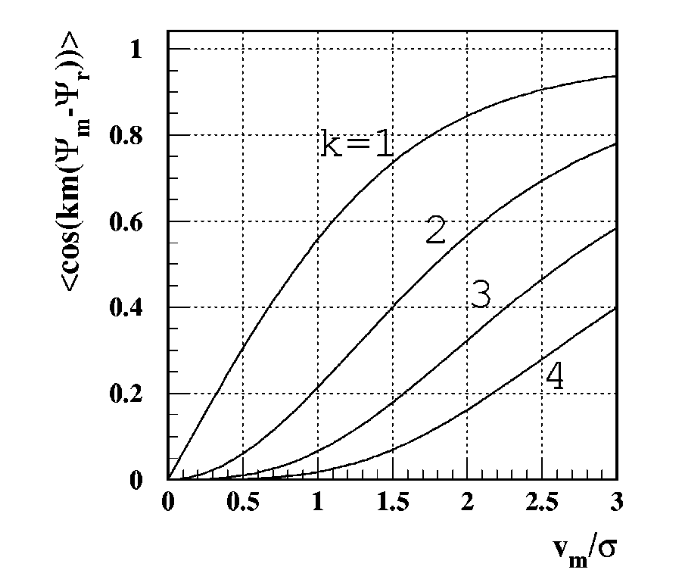
\includegraphics[scale=0.6]{chapter2/fig/resolution_vs_nu.png}
\caption{The event plane resolution for the $n^{th}$ (n=km) harmonic of the particle distribution with respect to the $m^{th}$ harmonic plane, as a function of $v_{m}$$/$$\sigma$.}
\label{fig:res_vs_nu} 
\end{figure}

Since we will use $\Psi_{1}$ to calculate $v_{1}$ and $v_{2}$, then we substitute (m=1, k=1) and (m=1, k=2) into the resolution equation to calculate the resolution for $v_{1}$ and $v_{2}$. $v_{1}$ and $v_{2}$ can be calculated with resolution shown in the following.

\begin{equation}
	R_{1} = \left< cos(\Psi_{1}-\Psi_{r}) \right>
	=\frac{\sqrt{\pi}}{2\sqrt{2}}\chi_{1}exp(-\chi_{1}^{2}/4) \times
	[I_{0}(\chi_{1}^{2}/4)+I_{1}(\chi_{1}^{2})/4]
	\label{equ:R1_chi1}
\end{equation}
\begin{equation}
	R_{12} = \left< cos(2(\Psi_{1}-\Psi_{r})) \right>
	=\frac{\sqrt{\pi}}{2\sqrt{2}}\chi_{1}exp(-\chi_{1}^{2}/4) \times
	[I_{1/2}(\chi_{1}^{2}/4)+I_{3/2}(\chi_{1}^{2})/4] 
	\label{equ:R12_chi1}
\end{equation}

\begin{equation}
	v_{1} =\frac{v_{1}^{obs}}{R_{1}} = 
	\frac{\left< cos(\phi-\Psi_{1}) \right>}{\left< cos(\Psi_{1}-\Psi_{r}) \right>}
\end{equation}
\begin{equation}
	v_{2} =\frac{v_{2}^{obs}}{R_{12}} = 
	\frac{\left< cos(2(\phi-\Psi_{1})) \right>}{\left< cos(2(\Psi_{1}-\Psi_{r})) \right>}
\end{equation}

Where the $R_{1}$ is the first order event plane resolution for $v_{1}$ and $R_{12}$ is second order event plane resolution estimated from first order event plane for $v_{2}$ calculation. In the equation \ref{equ:R1_chi1}, the $\chi_{1}$ is unknown. But we can first using three sub-event method to calculate the left hand first order event plane resolution ($R_{1}$), then we can determine the $\chi_{1}$, thus we substitute $\chi_{1}$ into equation \ref{equ:R12_chi1} to get the second order event plane resolution estimated from first order event plane for $v_{2}$ calculation ($R_{12}$). 

In the previous BES-I collider mode analysis, the resolution is determined from two sub-event method, which is required the multiplicity and flow signal of sub-events are same. This can be done by dividing the two sub-event from negative and positive $\eta$ range. But, if the sub-events are not "equal", or if we have only correlations between particles in different windows, and the resolution in each window can be different, then one needs at least three sub-events to determine the event plane resolution in each of them. In this case, the resolution in the first window is determined as:
\begin{equation}
	\left< cos(\Psi_{1}^{a}-\Psi_{r}) \right> = 
	\sqrt{\frac{\left< cos(\Psi_{1}^{a}-\Psi_{1}^{b}) \right>\left< cos(\Psi_{1}^{a}-\Psi_{1}^{c}) \right>}
	{\left< cos(\Psi_{1}^{b}-\Psi_{1}^{c}) \right>}}
\end{equation}
It's similar way to determine the other sub-event resolution. In this analysis, we divide the EPD to 4 sub-event groups, and we also combine the first two and last two group into one group, thus we have 6 sub-event groups and their resolution. as you can see in the figure \ref{fig:epd_1stres}, the first order event plane resolution as a function of centrality, different color and symbol means the same interest event plane resolution from different reference event plane. These difference will estimated into systematic uncertainties. From EPD-A to EPD-D, the resolution is decreasing with pseudorapidity decreases. This can be explained from that the $v_{1}$ signal is decreasing with pseudorapidity decreases.


\begin{figure}[ht]
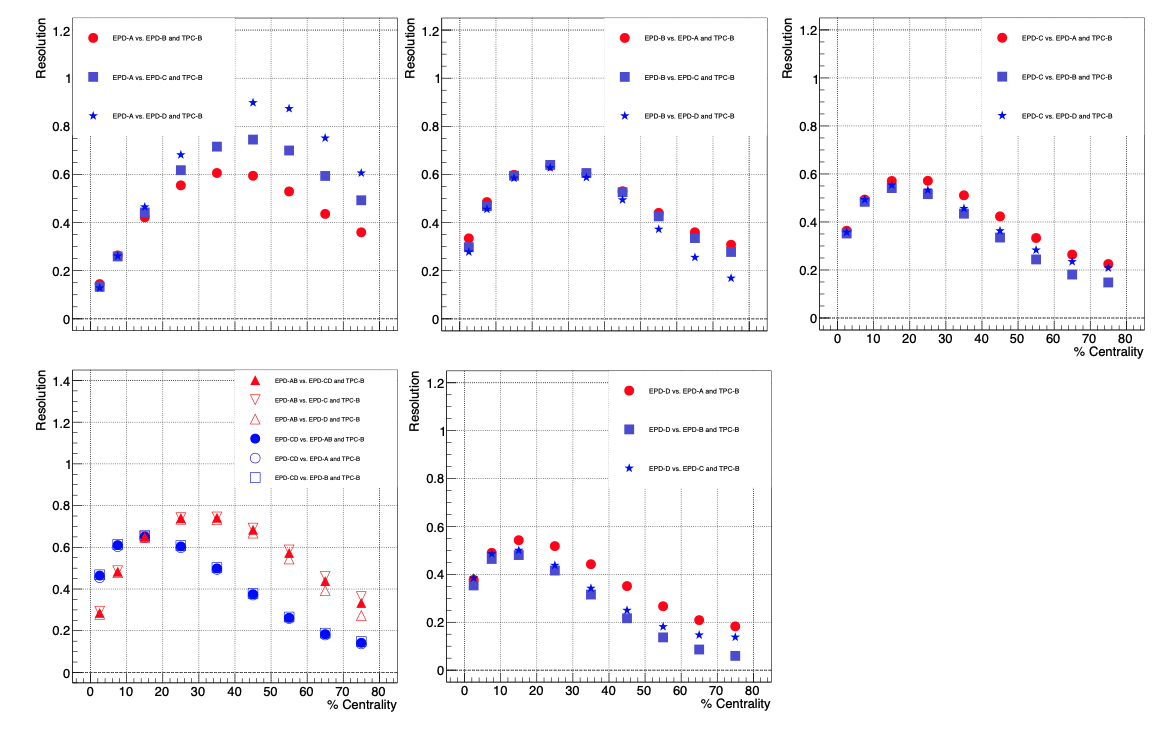
\includegraphics[scale=0.4]{chapter2/fig/epd_1stresolution.png}
\caption{ EPD First order event plane resolution as a function of centrality for different sub-event groups. Different symbol means the same interest event plane resolution using different reference event plane.}
\label{fig:epd_1stres}
\end{figure}



\subsection{Particle Identification}
\subsubsection{PID from TPC and TOF}
In this analysis, we use TPC and TOF detectors to identify particles (pion, kaon, and proton). Figure \ref{fig:dedx_mass2_3gev}, the left side, shows the TPC energy loss $dE/dx$ as a function of rigidity ($p/q$) with quality cuts. The curves for different color indicate the Bichsel expectation values for corresponding particles. As we can see, the TPC can identify particles at low momentum as illustrated by the color bands. At high momentum region, we need to identify particles together with TOF information. Figure \ref{fig:dedx_mass2_3gev}, the right side, shows the measured mass square as a function of rigidity ($p/q$) with track quality cuts. 

\begin{figure}[ht]
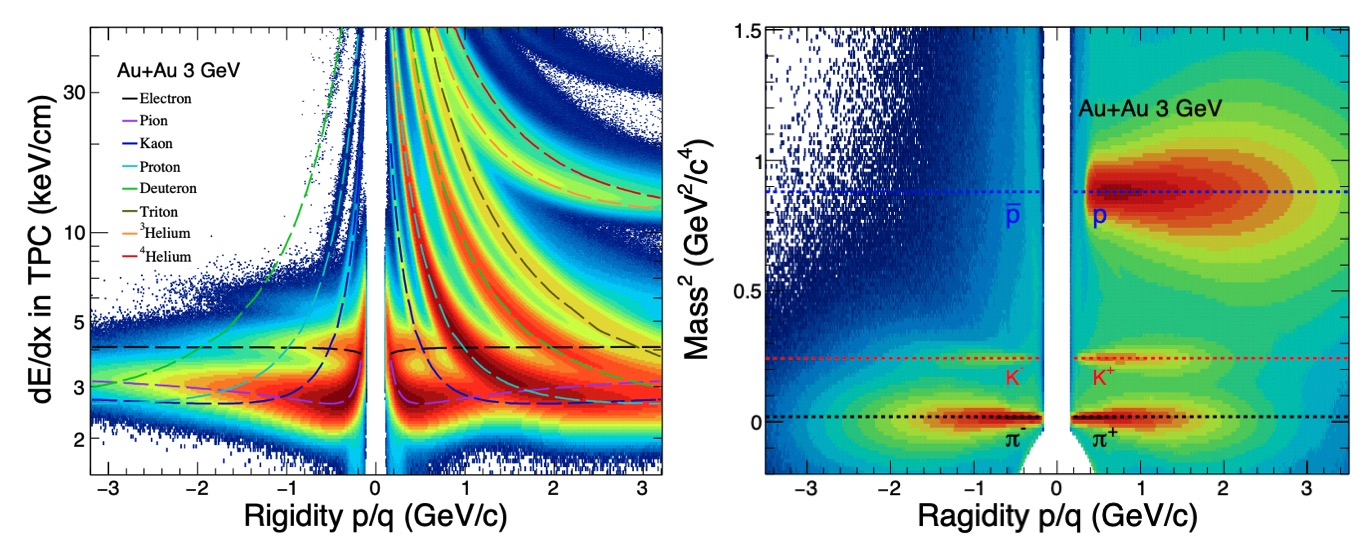
\includegraphics [scale=0.3]{chapter2/fig/dedx_3gev.png}
\caption{Left: Energy loss $dE/dx$ as a function of rigidity ($p/q$) for Au+Au collisions at $\sqrt{s_{NN}}$ = 3 GeV. The dash lines indicate the theoretical predicated values for different particles. Right: $Mass^{2}$ as a function of rigidity ($p/q$) for Au+Au collisions at $\sqrt{s_{NN}}$ = 3 GeV. The dash lines indicate the corresponding particles.}
\label{fig:dedx_mass2_3gev} 
\end{figure}

The $\left<dE/dx\right>$ distribution for a fixed particle type is not Gaussian. It has been shown that a better Gaussian variable, for a given particle type, is the $n\sigma_{particles}$, defined as:
\begin{equation}
	n\sigma_{particle} \propto ln \left[ \left< \frac{dE}{dX} \right>_{particle} / 
	\left< \frac{dE}{dX} \right>_{Bichsel} \right]
\end{equation}
where the particle type ($e^{\pm}, \pi^{\pm}, K^{\pm}, p, or  \bar{p}$) and $\left< \frac{dE}{dX} \right>_{Bichsel}$ is the corresponding Bichsel function. The most probable value of Bichsel function for the particle is 0.

The variable mass square ($m^{2}$) from TOF is given by:
\begin{equation} 
	m^{2} = p^{2} \left( \frac{c^{2}T^{2}}{L^{2}}-1 \right)
	\label{mass2_equ}
\end{equation}
where the p is the momentum, T is the time of travel by particle, L is the path length, and c is the speed of light.

\subsubsection{Acceptance of pion, kaon and proton}
In order to avoid fake tracks in the TPC and to improve the average momentum and energy loss resolution, the following track quality cuts in the table \ref{tab:tpc_cut_pid} were applied, then for the identification of pion, kaon and proton, we require TPC $n\sigma$ and TOF $mass^{2}$ cuts in the table \ref{tab:dedx_mass_cut_pid}. For pions and kaons, in addition of TPC $n_{\sigma}$ cut, we also apply TOF $m^{2}$ cut to improve their purity. For proton, since at 3GeV, the proton production will be dominated. So we only apply TPC $n_{\sigma}$ cut. Its purity is $>$ 90\% when the momentum $<$ 2GeV. After these cuts, these particles acceptance plot ($\pi^{\pm}, K^{\pm}$, p ) can be found in the figure \ref{fig:pikp_acceptance_fig}, we also label the target location at $y = -1.045$, as we can see, the acceptance for all particles cover midrapidity region, so that we can make a fair comparison with STAR high energy results.
 
 \begin{table}[ht]
\caption{\ TPC global tracks cuts for PID}
\label{tab:tpc_cut_pid}
\begin{tabular}{|c|c|}
\hline
nHitsFit$>$15 \\ \hline
nHitsFit/nHitsMax$>$0.52 \\ \hline
dca $<$ 3 (cm) \\ \hline
\end{tabular}
\end{table}


\begin{table}[ht]
\caption{\ dE/dX and $mass^{2}$ cut for PID}
\label{tab:dedx_mass_cut_pid}
\begin{tabular}{lclc|}
\hline
particle & cuts \\ \hline
pion  &  $|n\sigma_{\pi}|$ $<$ 3 and -0.1$<mass^{2}<$0.15 \\  \hline
kaon & $|n\sigma_{kaon}|$ $<$ 3 and 0.16$<mass^{2}<$0.36 \\ \hline
proton & $|n\sigma_{proton}|$ $<$ 2 \\ \hline
\end{tabular}
\end{table}

\begin{figure}[ht]
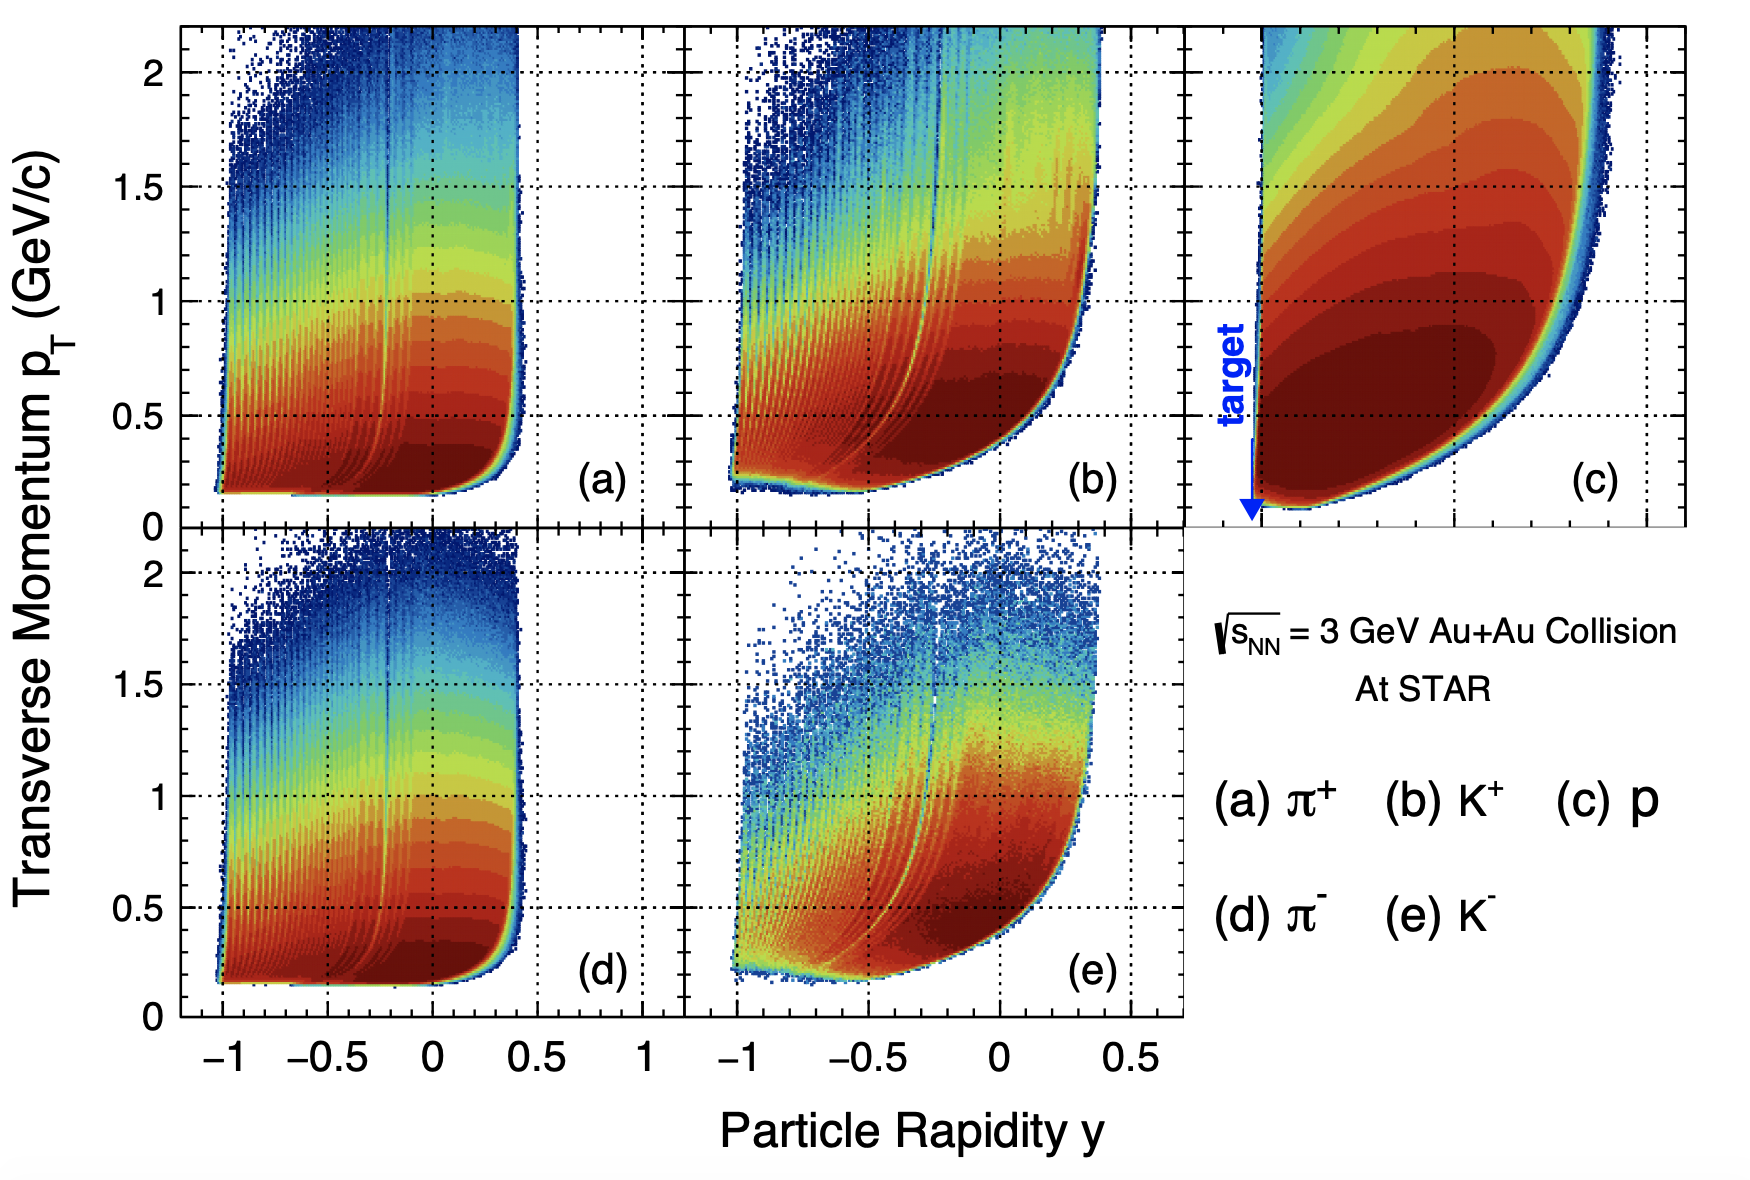
\includegraphics [scale=0.5]{chapter2/fig/pikp_acc_3gev.png}
\caption{ Rapidity(y) and transverse momentum($p_{T}$) acceptance of $\pi^{\pm}, K^{\pm}, proton$ using TPC and TOF in Au+Au collisions at $\sqrt{s_{NN}}$ = 3 GeV. The target is located at the y = -1.045. }
\label{fig:pikp_acceptance_fig}
\end{figure}

\clearpage
\newpage

\subsection{Efficiency Correction}

\subsubsection{TPC tracking efficiency}

The detector acceptance and the efficiency of reconstructing particle tracks are determined together by embedding Monte Carlo tracks simulated using the GEANT model \cite{Agostinelli:2002hh} of the STAR detector into real events at the raw data level. One important requirement is to have a match in the distributions of reconstructed embedded tracks and real data tracks for quantities reflecting track quality and used for track selection. The ratio of the distribution of reconstructed and original Monte Carlo tracks as a function of $p_{T}$ and rapidity gives the efficiency x Acceptance correction factor for the $p_{T}$ and rapidity interval studies. 
	
Figure \ref{fig:pikp_eff_tpc} shows the pion, kaon and proton TPC tracking efficiency as a function of $p_{T}$ and rapidity. In the FXT model collision, we do see efficiency alone the $p_{T}$ and rapidity direction. So, we plot the efficiency of particle species as a function of $p_{T}$ and rapidity. The track-by-track TPC tracking efficiency correction will be included in this analysis.

\begin{figure}
    \centering
    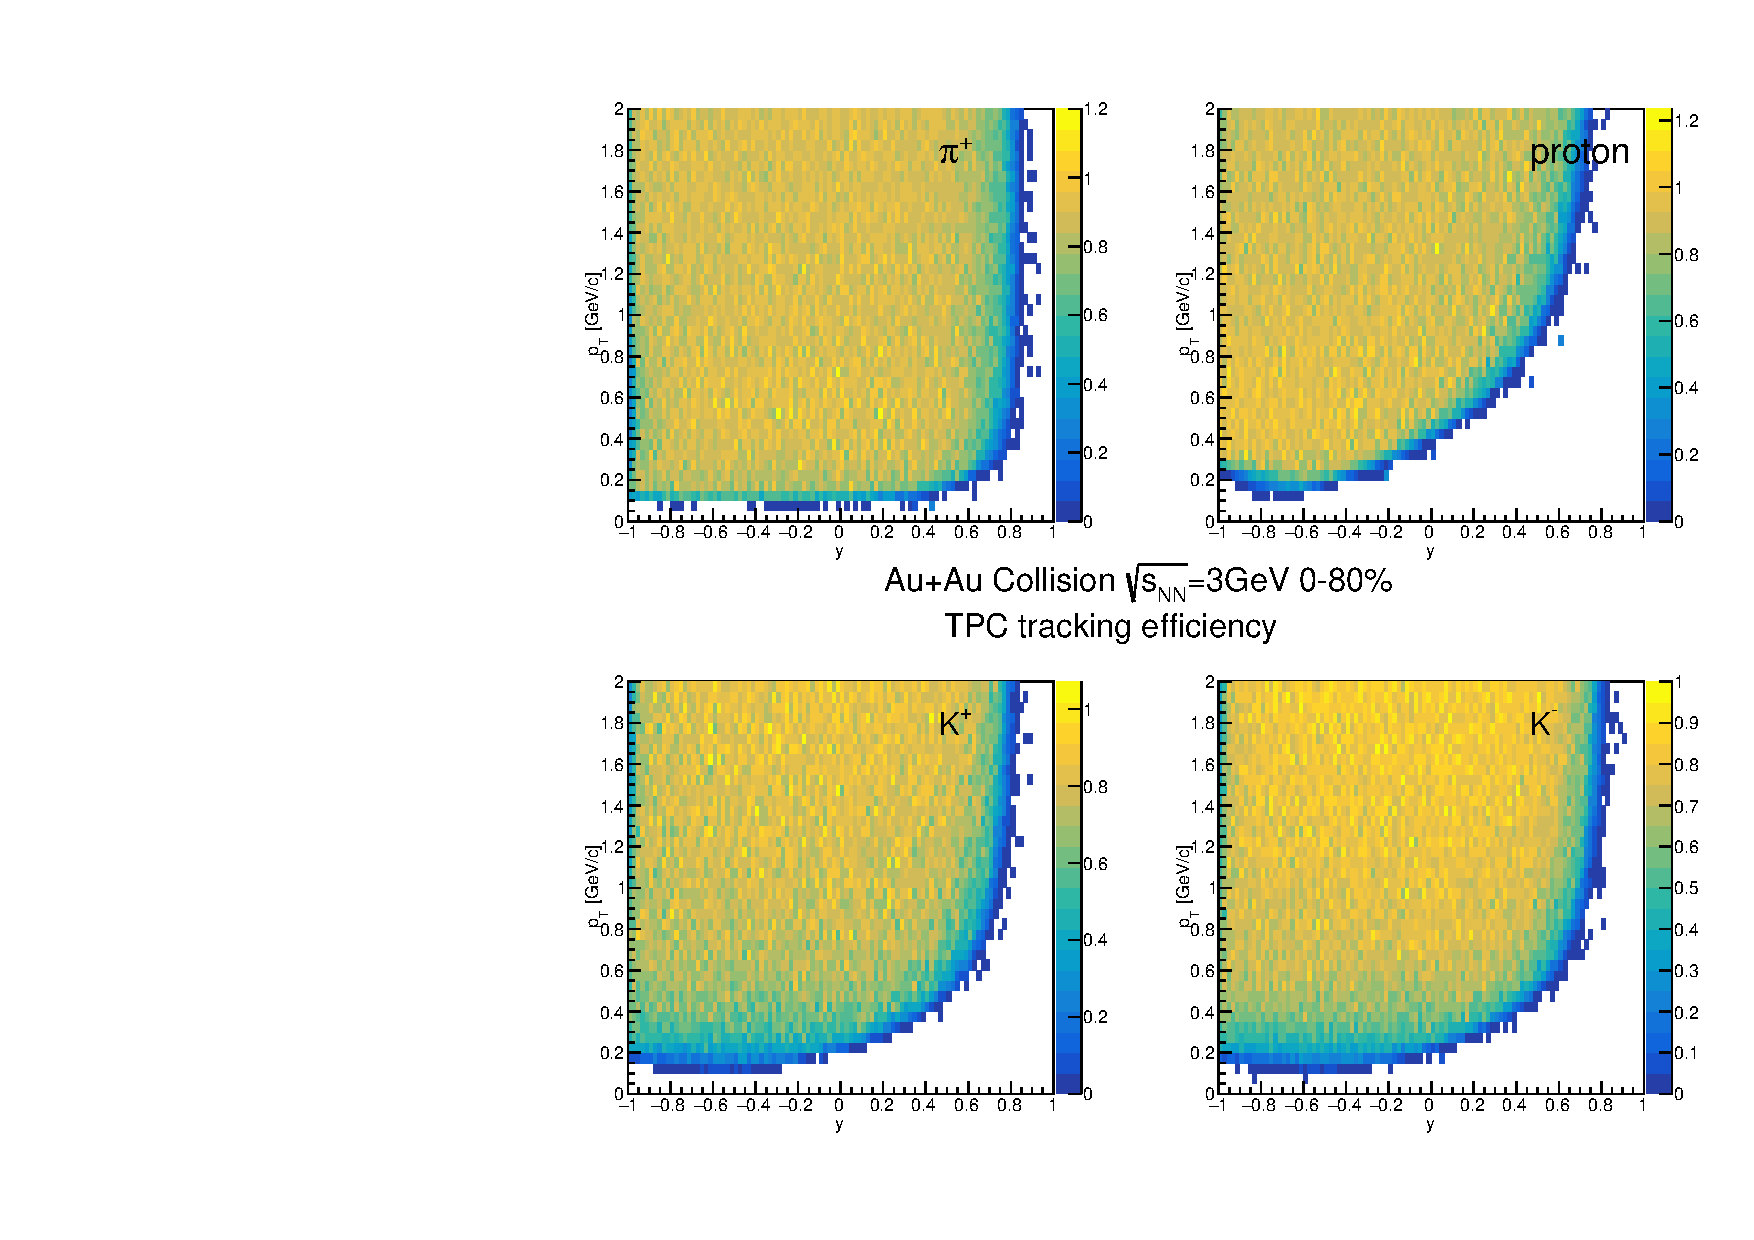
\includegraphics[scale=0.5]{FXT3gev/chapter2/fig/eff/pik_tpceff.pdf}
    \caption{pion, kaon, proton tracking efficiency as a function of $p_{T}$ and rapidity in 0-80\% for two-dimensional}
    \label{fig:pikp_eff_tpc}
\end{figure}
	
\subsubsection{TOF matching efficiency}

Since the TOF can give better particle identification than TPC at higher momentum region, however not all TPC tracks can travel into TOF and give a hit. So there is an extra correction called TOF matching efficiency correction used in our analysis. This is done with a data-driven technique. The TOF matching efficiency $\epsilon$ can be determined by number of TOF matched tracks divide by number of TPC tracks as shown in the formula \ref{equ:TOF_eff}. 
figure \ref{fig:pik_eff_tof} shows the two-dimensional efficiency as a function of $p_{T}$ and rapidity (y) in 0-80\% for pions and kaons. Since we give the additional $m^{2}$ cut for pions and kaons.
The track-by-track TPC tracking associated TOF matching efficiency correction will be applied into our analysis.

\begin{equation}
    \epsilon (p_{T}, y) = \frac{\text{Number of TOF Matched Tracks}}{\text{Number of TPC Tracks}}
    \label{equ:TOF_eff}
\end{equation}

\begin{figure}
    \centering
    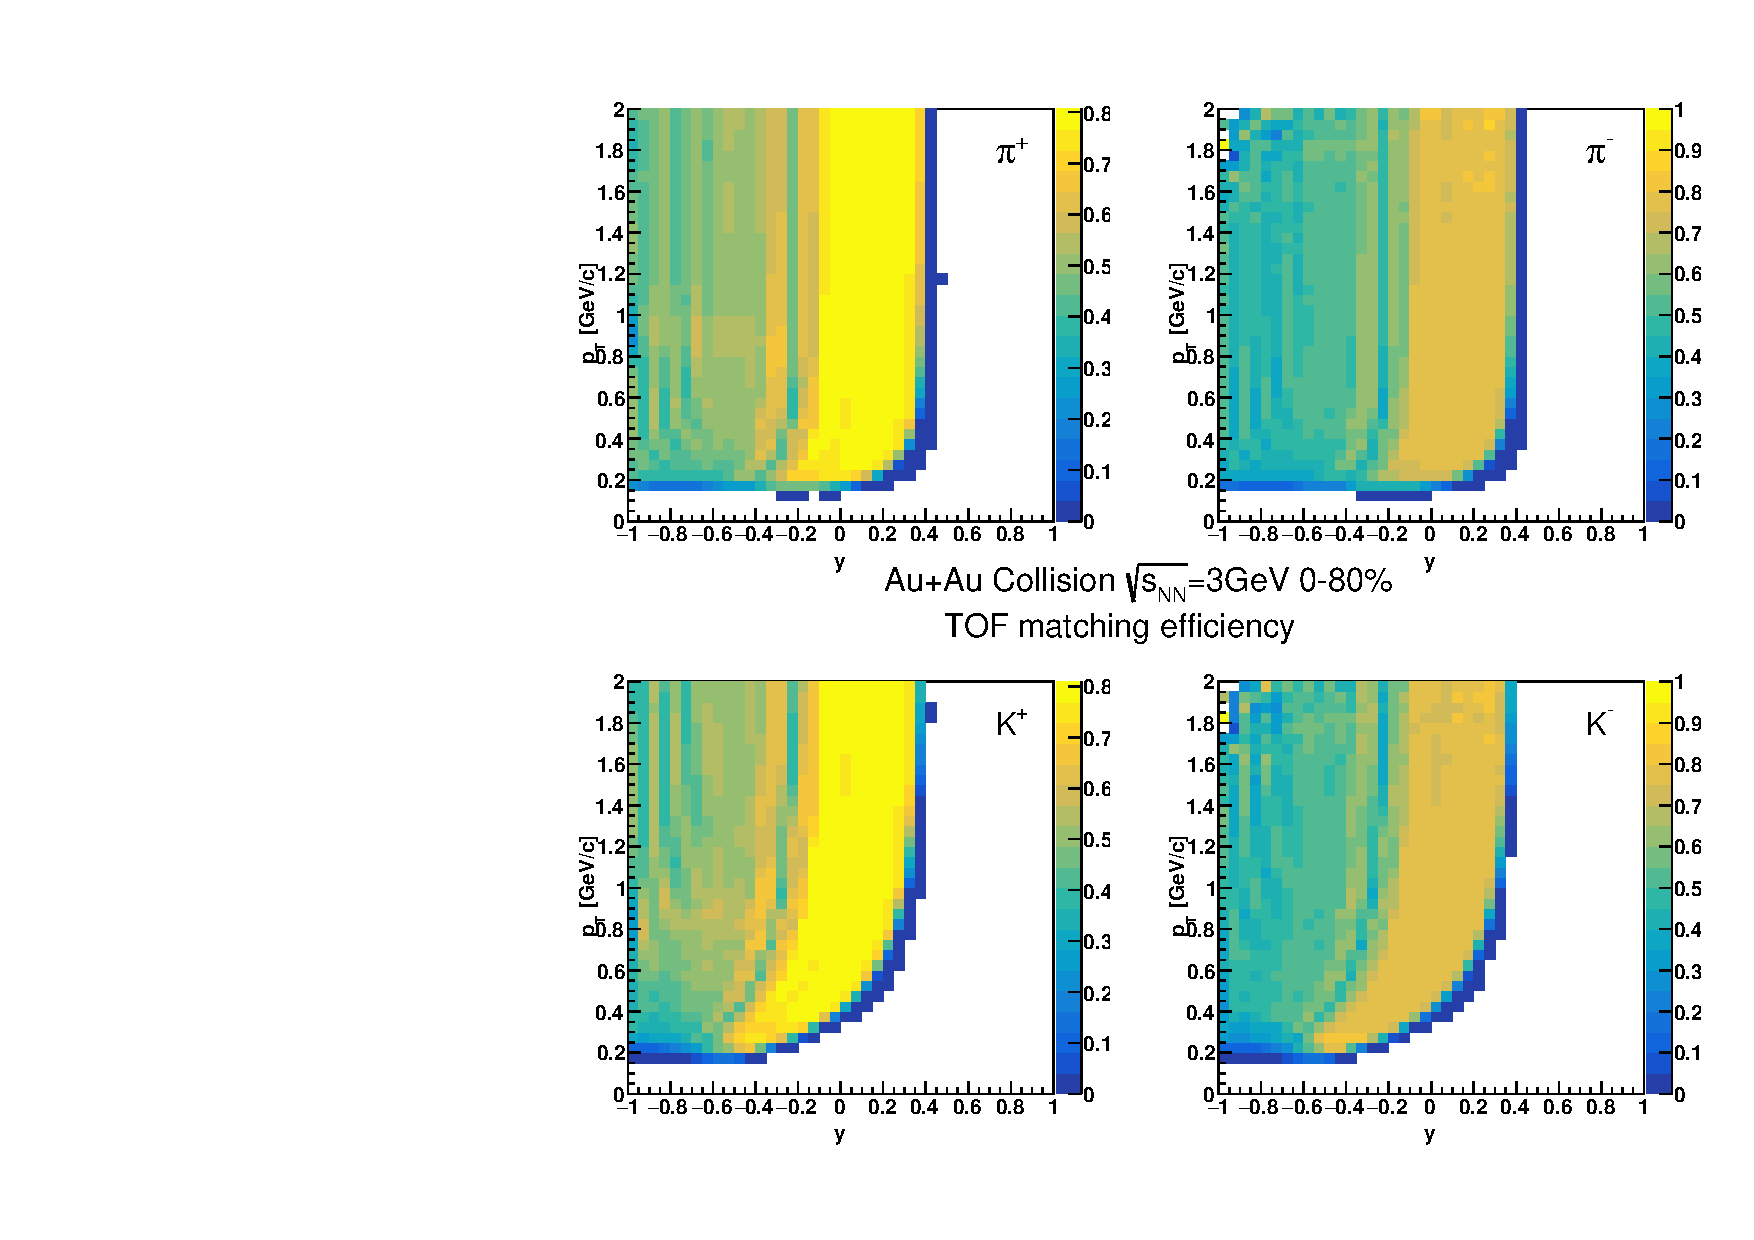
\includegraphics[scale=0.5]{FXT3gev/chapter2/fig/eff/pik_tofeff.pdf}
    \caption{pion, kaon TOF matching efficiency as a function of $p_{T}$ and rapidity in 0-80\% for two-dimensional}
    \label{fig:pik_eff_tof}
\end{figure}

